Let $d_{j,i}$ denote the distance from vertex $P_i$ to focus $f_j$ of $\E$.

\begin{proposition}
Over the homothetic family, $\sum_i{d_{1,i}}$ and $\sum_i{d_{2,i}}$ are equal and invariant.
\label{prop:dist-focus}
\end{proposition}

\begin{proof}
\textcolor{red}{Sergey}
\end{proof}

Since for an ellipse $\kappa_i=(a b)^{2/3} d_{1,i} d_{2,i}$, then:

\begin{corollary}
Over the homothetic family, the quantity $\sum_{i=1}^N{\kappa_i^{-2/3}}$ is invariant.
\label{cor:kappa}
\end{corollary}

\begin{figure}
    \centering
    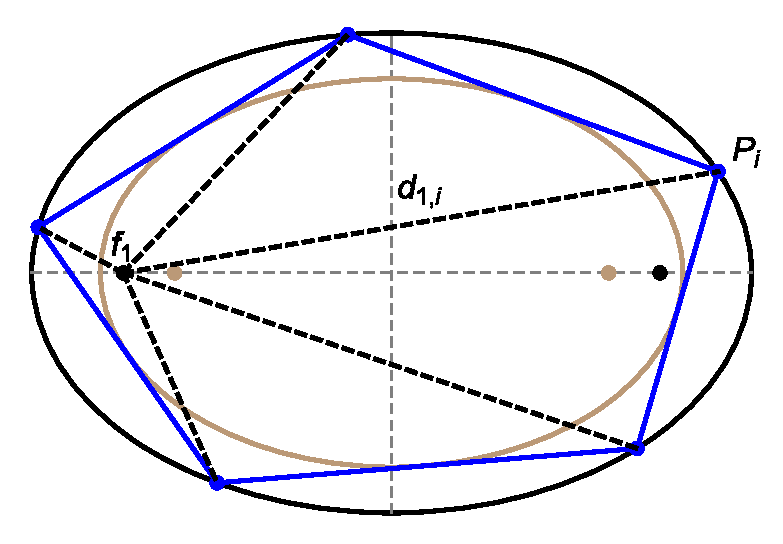
\includegraphics[width=.6\textwidth]{pics/0060_spoke_sum.eps}
    \caption{Over the homothetic family, the sum of distances $d_{1,i}=|P_i-f_1|$ is invariant, where $f_1$ is a focus of the outer ellipse.}
    \label{fig:spoke-sum}
\end{figure}